\documentclass[11pt,a4paper]{article}
\usepackage[margin=1in]{geometry}
\usepackage{graphicx}
\usepackage{booktabs}
\usepackage{hyperref}

\title{CMPE476 --- C10K Project: Benchmark Report\\
\large Comparing Thread-per-Connection vs. Epoll Event-Loop Servers}
\author{YOUR NAME HERE --- Student ID: XXXXXXX}
\date{\today}

\begin{document}

\maketitle

\section{Introduction}
This report presents benchmark results for two concurrent TCP server implementations developed for the CMPE476 C10K project: a traditional thread-per-connection server (\texttt{threadserv}) and a high-performance single-threaded epoll-based event-loop server (\texttt{epollserv}). Both servers implement the same line-based text protocol and were tested under identical load conditions using the provided \texttt{client\_flood} tool. The goal of this report is to quantify the architectural trade-offs discussed in Chapter 2 of the course, particularly memory footprint scaling and throughput scalability.

\section{Test Setup}
All experiments were conducted on a single machine with the following configuration:
\begin{itemize}
    \item \textbf{Machine:} Intel(R) Core(TM) i7-14650HX, 32 GB RAM
    \item \textbf{Operating System:} Ubuntu 24.04.4 LTS (via WSL2)
    \item \textbf{Kernel Version:} 6.6.87.2-microsoft-standard-WSL2
    \item \textbf{File Descriptor Limit:} \texttt{ulimit -n 65535}
    \item \textbf{sysctl tuning:} No additional \texttt{sysctl} parameters were modified beyond defaults.
\end{itemize}
Both servers and the \texttt{client\_flood} load generator were run on the same host, communicating over the localhost loopback interface (\texttt{127.0.0.1}).

\section{Methodology}
The \texttt{client\_flood} tool was used to establish $N$ concurrent connections ($N = 1{,}000$, $5{,}000$, and $10{,}000$), with each connection sending $M=20$ PING requests. Wall-clock time was measured for the full flood, and Requests Per Second (RPS) was calculated as the total completed requests divided by the elapsed seconds. Memory (VmRSS and VmSize) was sampled from \texttt{/proc/<pid>/status} at peak load using a separate hold-connection experiment that kept all $N$ connections open for 12 seconds.

\section{Results}

\subsection{Throughput Comparison}
Table 1 shows the throughput performance in Requests Per Second (RPS) for both server architectures.

\begin{table}[h]
\centering
\begin{tabular}{lrrrrrr}
\toprule
\textbf{Server} & \textbf{Clients} & \textbf{Req/Client} & \textbf{Completed} & \textbf{Failed} & \textbf{Elapsed (s)} & \textbf{RPS} \\
\midrule
threadserv & 1,000  & 20 & 20,000  & 0 & 0.101 & 197,742 \\
threadserv & 5,000  & 20 & 100,000 & 0 & 1.147 & 87,177  \\
threadserv & 10,000 & 20 & 200,000 & 0 & 5.220 & 38,313  \\
\midrule
epollserv  & 1,000  & 20 & 20,000  & 0 & 0.052 & 383,745 \\
epollserv  & 5,000  & 20 & 100,000 & 0 & 0.245 & 408,229 \\
epollserv  & 10,000 & 20 & 200,000 & 0 & 0.845 & 236,653 \\
\bottomrule
\end{tabular}
\caption{Throughput benchmark results}
\end{table}

\subsection{Memory Comparison}
Table 2 details the peak memory footprint, highlighting both Resident Set Size (RSS) and Virtual Memory Size (VmSize).

\begin{table}[h]
\centering
\begin{tabular}{lrrrr}
\toprule
\textbf{Server} & \textbf{Clients} & \textbf{Peak RSS (MB)} & \textbf{Peak VmSize (MB)} \\
\midrule
threadserv & 1,000  & 7.88  & 8,006.79  \\
threadserv & 5,000  & 40.50 & 40,023.44 \\
threadserv & 10,000 & 80.06 & 80,044.39 \\
\midrule
epollserv  & 1,000  & 3.38  & 4.55  \\
epollserv  & 5,000  & 11.25 & 12.42 \\
epollserv  & 10,000 & 21.19 & 22.34 \\
\bottomrule
\end{tabular}
\caption{Memory footprint benchmark results}
\end{table}

\begin{figure}[h]
    \centering
    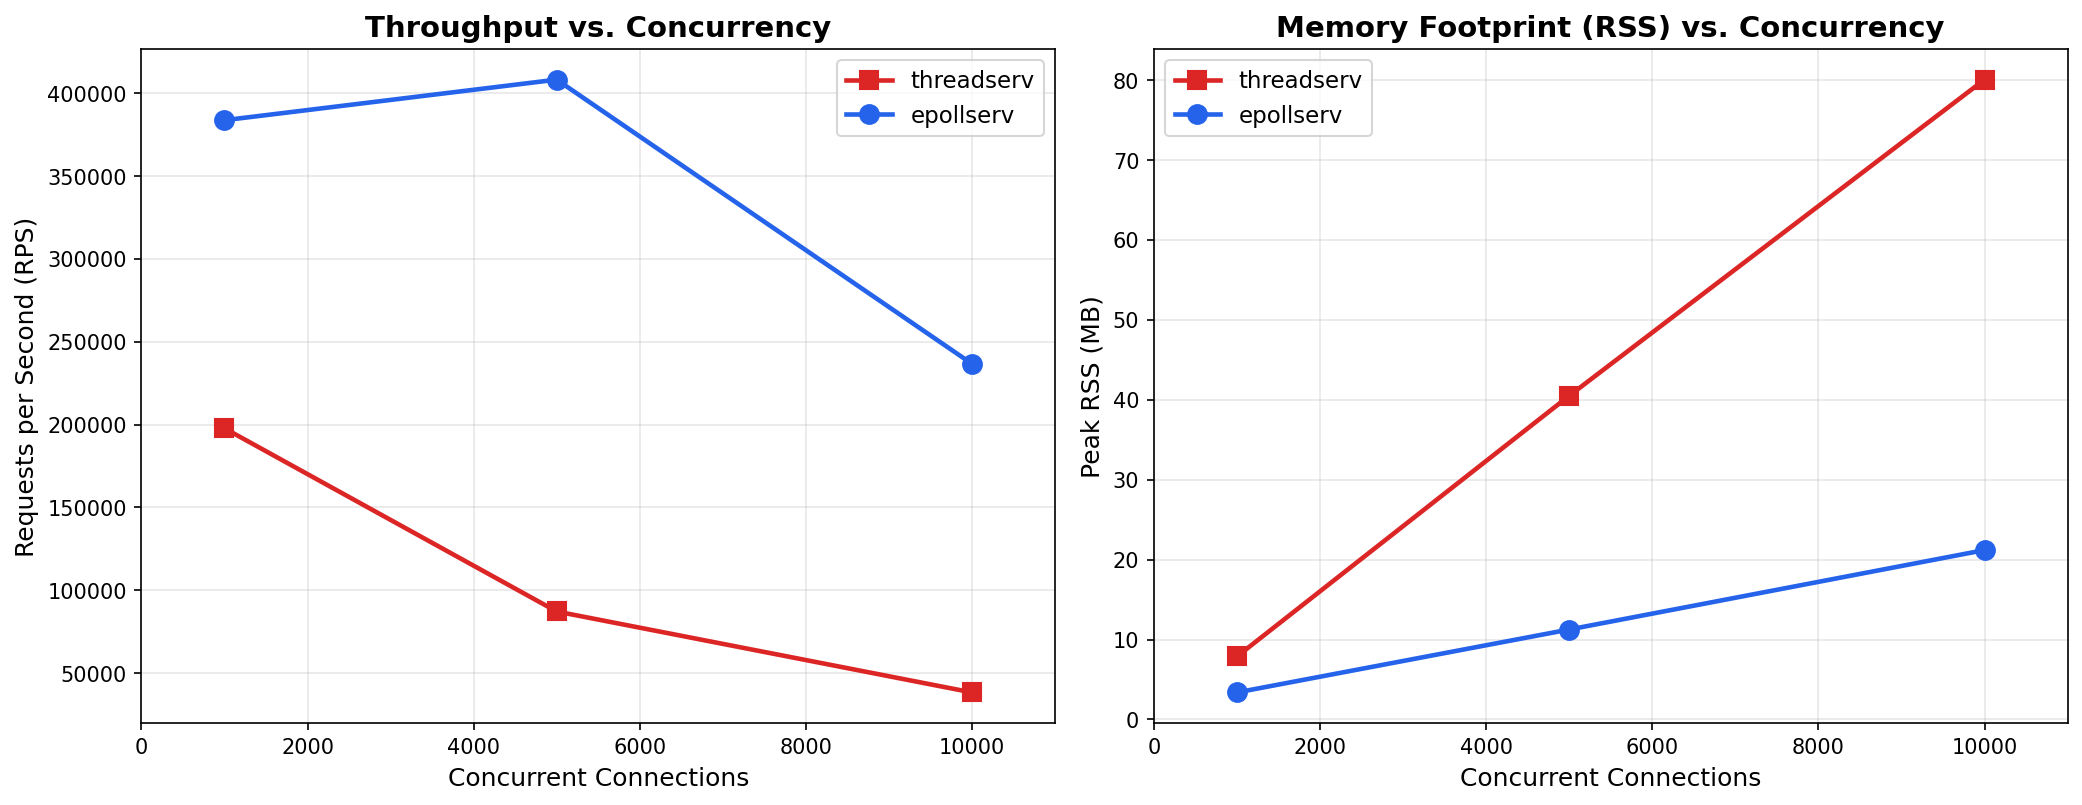
\includegraphics[width=0.95\textwidth]{benchmark_chart.png}
    \caption{Throughput and Memory (RSS) scaling as concurrent connections increase.}
    \label{fig:chart}
\end{figure}

\section{Analysis}

\paragraph{Throughput:} The \texttt{epollserv} vastly outperforms the \texttt{threadserv} as concurrency scales. While \texttt{threadserv} drops significantly from roughly 197k RPS down to 38k RPS at 10,000 connections, \texttt{epollserv} sustains incredibly high throughput (peaking over 400k at 5k clients and remaining at 236k at 10k clients). The thread-per-connection model slows down under high concurrency primarily due to the severe context-switching overhead incurred by the kernel scheduling thousands of runnable threads.

\paragraph{Memory and the C10K Problem:} The memory footprint results precisely illustrate the C10K challenge. For \texttt{threadserv}, while the actively paged physical memory (RSS) scales reasonably (up to 80 MB for 10k connections due to lazy allocation), the Virtual Memory (VmSize) absolutely explodes, reaching an astounding 80 GB at 10,000 connections. This occurs because every new POSIX thread allocates a default stack (typically 8 MB on Linux), meaning 10,000 threads reserve $10{,}000 \times 8 \text{ MB} \approx 80 \text{ GB}$ of address space. In stark contrast, \texttt{epollserv} gracefully handles 10,000 connections using only around 22 MB of virtual space and physical RAM combined, allocating only small \texttt{client\_t} structs and connection buffers in a single address space.

\section{Limitations}
All benchmarks were executed on the localhost loopback interface, which eliminates real network latency, packet loss, and TCP round-trip delays. In a production scenario over a physical network, the throughput gap between the two architectures would likely narrow because I/O wait times would dominate over CPU-level scheduling overhead. Additionally, the \texttt{client\_flood} generator and the server share the same CPU and memory resources, which introduces resource contention that would not exist in a true client--server deployment. The results should therefore be interpreted as a comparison of architectural overhead rather than absolute production performance.

\section{Conclusion}
The experimental results strongly validate the C10K theories discussed in class. Relying on POSIX threads per connection is fundamentally unscalable past a few thousand connections due to excessive stack memory reservations and kernel context-switching latency. Conversely, an event-driven, single-threaded architecture utilizing \texttt{epoll} effectively bypasses these bottlenecks, providing a robust, highly scalable, and memory-efficient solution for massive concurrency.

\end{document}
